\title{\huge dSoftArk \\
       \small Afleveringsopgave - uge 2 genaflevering - MultiCiv}
\author{Hold: DA4; Gruppe: B\\ \\
        \href{mailto:skeen@cs.au.dk}{Emil Madsen - 20105376}\\
        \href{mailto:emray@cs.au.dk}{Rasmus - 20105109}\\
        \href{mailto:sverre@cs.au.dk}{Sverre - 20083549}
       }
\date{\today}

\maketitle

\hrule

\section*{ Changes since the intial handin }
In our original handin we didn't not have a solution to exercise 36.11.
We do not have a solution this week either, as the exercise was discussed in class. 
However a new UML diagram reflection our changes has taken the place of the old world and is found in the last section of this document.

As for the misunderstanding of the Strategy Pattern, we must admit that we did
not misunderstand the strategy pattern, but chose to use inheritance
instead, simply because it seemed a better design at the time.
The class review of exercise 36.11 changed our minds about that, however, and in this new handin we've changed the design to something more 'strategeekish'.

We've effectively created 3 interfaces:
one for unit actions, 
one for unit movement 
and 
one for unit attacks. 

These are obviously implemented as strategy patterns, as reflected by our UML diagram. 
And as such there is only 4 strategies implemented for all of our units (3 defaults and a gammasettler (build city) strategy). 

Beside this, we chose to go with a decorator pattern for the gamma archer, simply because all it does is change the behavior of some underlaying strategy. 

We decided to go with this strategy pattern implementation instead of a more faking hardcode-it implemenation, simply because we wanted to keep our code flexiable and keep GameImpl clear of variant specific code.

We've also decided to keep our unit actions on the units, as we found that to be the most intuitive and flexible solution,
We see it in the way that "Units perform the action", not "The game perform an action with a unit".

Please do note that we've removed the UnitStrategy interface, and replaced it
with the 3 previously mentioned ones. where most of these have been implemented with the default.

And we made sure to implement it more strategy patternish, instead of inheritanceish. 
Also Unit abstractions is gone, as the entire earlier Unit Class System is gone.
\\

As mentioned in our feedback in class, we choose to get rid of all our *Ext interfaces, but to keep the isolation level we wanted, we have decided to split our
interfaces into readonly, and modifyable interfaces, such that mutators on Unit/Tile, ect. only are accessible by those who need the modifiable interface.
Fx not the gui, as that will have to operate using game (non modifiable) interface.
\\

We've also renamed our StrategyPack's to StrategyFactories, as that's what they
really are.

As for rewriting our testcases, we've decided not to do so, for the current
code, but instead to apply the feedback, for the upcoming iterations. 

This is simply to save time and is a matter of prioritising the items on our backlog higher.


The TestHelper.runOneRound() method, was changed, to run until a player in
turn, gets the turn again, such that it still works for x players, however
without relying on the age, and now it does actually run a complete round,
instead of just running till roundstart. - As one would expect.


As for the implementation of deltaciv:
We didn't notice the issue, and this has been fixed, such that worlds are now dynamically loaded based upon a string (As given with the provided example code).

    
As for the inheritance between our factories:
We've decided to keep that, but rename Alphaciv into a defaultciv, that holds the common default behavier between the different variants. 
As such, we've decided to go with some limited inheritance, such that we simply overload the strategies we want to specify, and unspecified defaults to alphaciv.
This is by design, to remove the amount of code duplication.


As a last note:
We've choosen to move all our GameConstants, into GameConstants,
   for instance ARCHER\_ATTACK and such.
However these values are not used
   anywhere, as the requirements does not state that the GammaArcher should
   have a positive attack rating.
It just states that it should double it's attack rating.

\section*{
A short outline of the TDD refactoring iteration that refactors your AlphaCiv variant into a design that will support the BetaCiv requirement (not the actual BetaCiv feature adding iteration!) }
\begin{comment}
A short outline of the TDD refactoring iteration that refactors your AlphaCiv variant into a design that will support the BetaCiv requirement (not the actual BetaCiv feature adding iteration!) }
\end{comment}

\begin{comment}
Thise are some exerpts from our devlog describing refactoring steps from our development on our:


\logInputfile{39}{42}{../../BetaCiv/Devlog.txt}
\logInputfile{51}{76}{../../BetaCiv/Devlog.txt}

So we basically just implemented the betaciv getWinner() in a strategy pattern, and, because the implementing strategy required knowledge about the the age of game, we let the strategy require a parameter specifying the age.

% iterationen for nogle af de test i de andre iterationer, 

% 12345 punkterne for de nye test,

\end{comment}

This weeks TDD iteration includes a lot of refactoring and variability handling.

Last week we earned confidence in our coding capability and this have allowed us to more radically restructure our code and more efficiently introduce strategy pattern as a solution to variability handling.

To get ready to the new weeks work we did some small stuff, like:
\begin{enumerate} \itemsep1pt \parskip0pt \parsep0pt
\item Forking the repository AlphaCiv branch into a Multiciv branch and closing the AlphaCiv branch
\item Renaming the source directory from standard to common
\item Setup new folder: hotciv.variants.alphaciv, with the testcase, TestAlphaCiv, in.
\item Adding new testcase, TestBetaCiv, in a new folder: hotciv.variants.betaciv.
\item Editing build.xml as necessary.
\end{enumerate}

The editing of build.xml allowed us to start writing testcases for betaciv and every time we ran Ant on our source, Ant would show os status on both betaciv and alphaciv.

Our refactoring on the common source (from the development on AlphaCiv) included changes to the constructor in GameImpl to accept paremeters that is used to specify how to execute getWinner(). 
The existing code in getWinner where moved to the parameter object and thus called via that object.


\section*{ A short outline of the variability points you have identified for Beta-, Gamma-, and DeltaCiv. }
% A short outline of the variability points you have identified for Beta-, Gamma-, and DeltaCiv. 
We found the following variability points on the different versions of multiciv:

\begin{verbatim}
            Alpha   Beta    Delta   Gamma
getWinner   common  variant common  common
getAge      common  variant common  common
worldSetup  common  common  variant common
unitAction  common  common  common  variant
\end{verbatim}

\subsection*{ 3-1-2 process for one of the variants. For one of them, discuss the use of the 3-1-2 process and the Strategy pattern. }
%  3-1-2 process for one of the variants. For one of them, discuss the use of the 3-1-2 process and the Strategy pattern. 

\subsubsection*{ \raisebox{.5pt}{\textcircled{\raisebox{-.9pt} {3}}} - Identifying behavior that varies}

In betaciv we first encountered a need for a different demand set for winning.
The new demand set was a need for a single player to own all existing cities. 
This is a demand set that is likely to change. 
Fx could another demand be that the players must vote every 4 rounds to possible decide a game winner, and only by majority vote can a winner be found.


\subsubsection*{ \raisebox{.5pt}{\textcircled{\raisebox{-.9pt} {1}}} - Stating the responsibility in an interface}

The only place the functionality differs, is in Game.getWinner(), and we rewrite the method like this:

\begin{lstlisting}
public Player getWinner()
{
    return winStrategy.getWinner();
}
\end{lstlisting}

Then we need the interface to be like this:
\begin{lstlisting}
public interface WinStrategy
{
    public Player getWinner();
}
\end{lstlisting}

\subsubsection*{ \raisebox{.5pt}{\textcircled{\raisebox{-.9pt} {2}}} - Composing the behavior by delegation}

In the attempt to compose the delegated behavior, we stumble upon a problem.
The behavior needs to know about part of the state of the game, namely the age, and in the case of the new variant, also the ownership of the cities.
They are accessible through the method Game.getAge() and Game.getCityAt().getOwner().

We chose to seed the game-state to the interface as a parameter to getWinner().
The interface looks like this now:
\lstinputlisting[linerange=5-14]{../../hotciv/src/hotciv/framework/strategy/WinStrategy.java}


\section*{ An UML class diagram outlining the final compositional design including all variants.}
This is the UML class diagram: \\
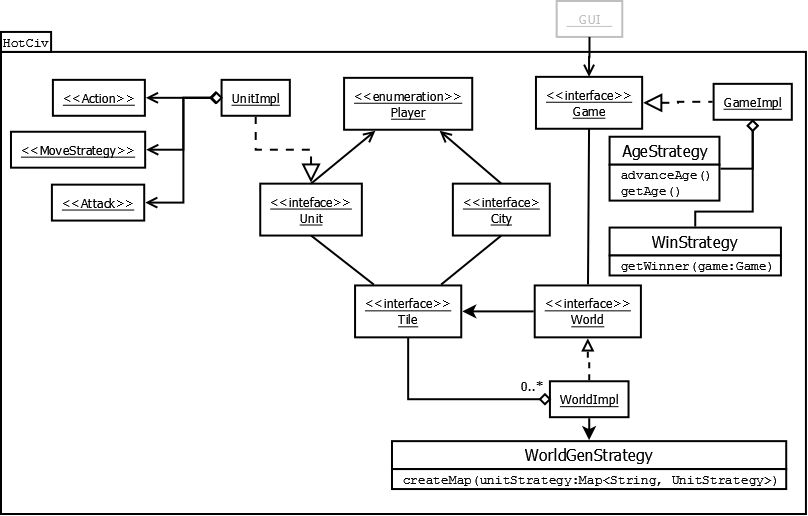
\includegraphics[width=\textwidth]{../UML_u2}



